% 摘录自https://tex.stackexchange.com/questions/515625/draw-derivative-tangent-at-specific-point-in-tikz
\documentclass[tikz,border=3mm]{standalone}

\usepackage{ctex}% 支持中文

\usetikzlibrary{intersections}

\usetikzlibrary{decorations.markings}
\tikzset{tangent/.style={% https://tex.stackexchange.com/a/25940
        decoration={
            markings,% switch on markings
            mark=
                at position #1
                with
                {
                    \coordinate (tangent point-\pgfkeysvalueof{/pgf/decoration/mark info/sequence number}) at (0pt,0pt);
                    \coordinate (tangent unit vector-\pgfkeysvalueof{/pgf/decoration/mark info/sequence number}) at (1,0pt);
                    \coordinate (tangent orthogonal unit vector-\pgfkeysvalueof{/pgf/decoration/mark info/sequence number}) at (0pt,1);
                }
        },
        postaction=decorate
    },
    use tangent/.style={
        shift=(tangent point-#1),
        x=(tangent unit vector-#1),
        y=(tangent orthogonal unit vector-#1)
    },
    use tangent/.default=1}

\begin{document}

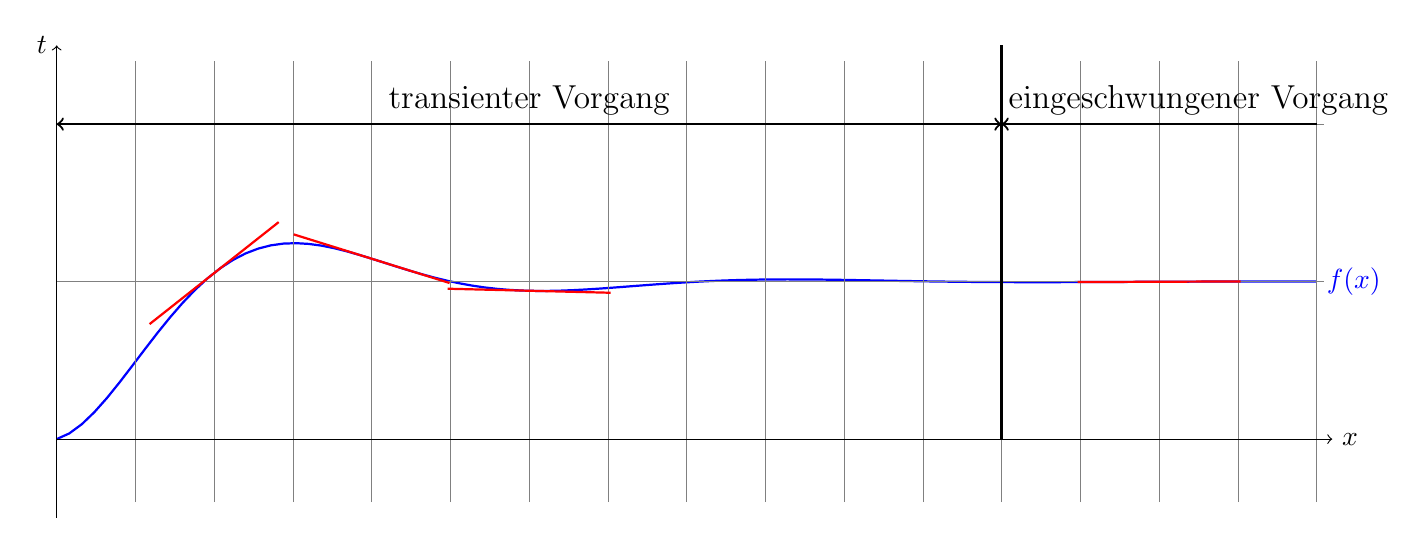
\begin{tikzpicture}[yscale=2,domain=0:16,samples=101,
pics/tangent at/.style={code={
    \path[name path=l] (#1*1cm-1pt,0|-current bounding box.south)
      -- (#1*1cm-1pt,0|-current bounding box.north);
    \path[name path=r] (#1*1cm+1pt,0|-current bounding box.south)
      -- (#1*1cm+1pt,0|-current bounding box.north);
    \draw[pic actions,
        name intersections={of=\pgfkeysvalueof{/tikz/tangent pic/graph name} and l,by=li},
        name intersections={of=\pgfkeysvalueof{/tikz/tangent pic/graph name} and r,by=ri}]
       (li) -- (ri);}},
tangent pic/.cd,graph name/.initial=graph]
      \draw[blue,thick,name path=graph] plot (\x,{1-exp(-0.45*\x)*(cos(deg(sqrt(1-0.0001)*\x))+0.3/(sqrt(1-0.2^2))*sin(deg(sqrt(1-0.1^2)*\x)))}) node[right] {$f(x)$};
      \draw[very thin,gray] (0,-0.4) grid (16.1,2.4);
      \draw[->] (0,0) -- (16.2,0) node[right] {$x$};
      \draw[->] (0,-0.5) -- (0,2.5) node[left] {$t$};
      \draw[black,<->,thick] (0,2) -- (12,2);
      \draw[black,thick] (6,2.15) node[font=\large]{transienter Vorgang};
      \draw[black,<-,thick] (12,2) -- (16,2);
      \draw[black,thick] (14.5,2.15) node[font=\large]{eingeschwungener Vorgang};
      \draw[black,-,thick] (12,2.5) -- (12,0); 
      \path foreach \X in {2,4,6,14}
      {pic[red,thick,shorten <=-1cm,shorten >=-1cm]{tangent at=\X}};
    \end{tikzpicture}

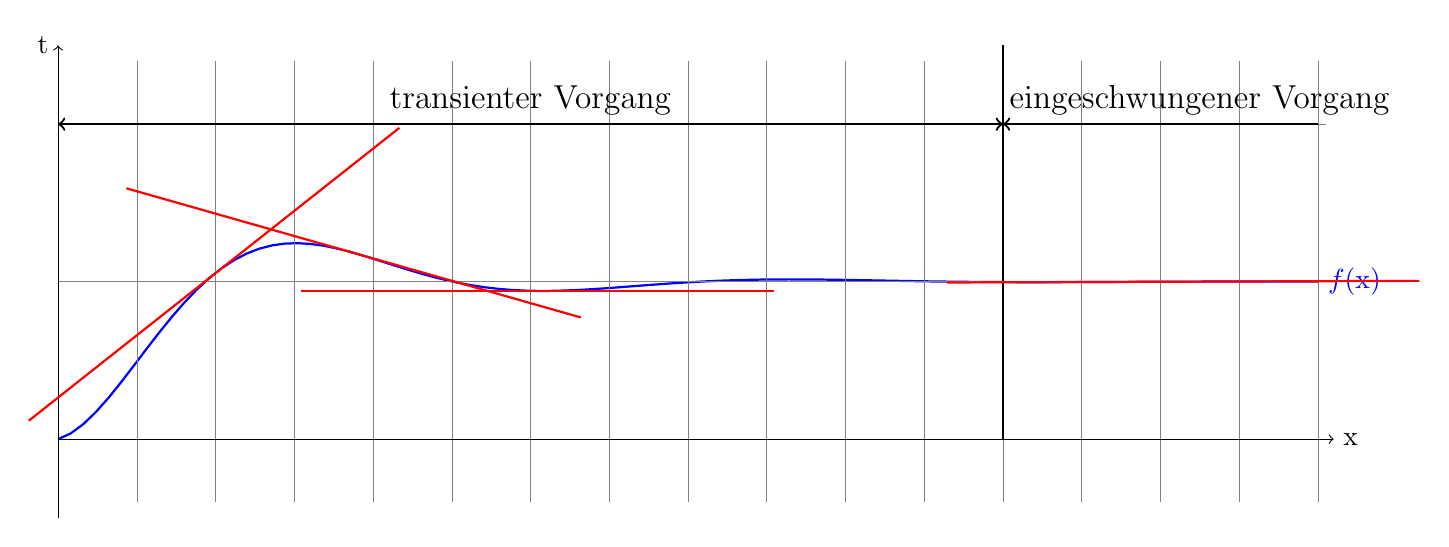
\begin{tikzpicture}[yscale=2,domain=0:16,samples=101]
      \draw[blue,thick,tangent/.list={0.17,0.28,0.42,0.9}] plot (\x,{1-exp(-0.45*\x)*(cos(deg(sqrt(1-0.0001)*\x))+0.3/(sqrt(1-0.2^2))*sin(deg(sqrt(1-0.1^2)*\x)))}) node[right] {$f(\mathrm{x})$};
      \draw[very thin,gray] (0,-0.4) grid (16.1,2.4);
      \draw[->] (0,0) -- (16.2,0) node[right] {$\mathrm{x}$};
      \draw[->] (0,-0.5) -- (0,2.5) node[left] {$\mathrm{t}$};
      \draw[black,<->,thick] (0,2) -- (12,2);
      \draw[black,thick] (6,2.15) node{{\large $\mathrm{transienter}\,\,\mathrm{Vorgang}$}};
      \draw[black,<-,thick] (12,2) -- (16,2);
      \draw[black,thick] (14.5,2.15) node{{\large $\mathrm{eingeschwungener}\,\,\mathrm{Vorgang}$}};
      \draw[black,-,thick] (12,2.5) -- (12,0); 
      \foreach \X in {1,...,4}
      {\draw [red, thick, use tangent=\X] (-3,0) -- (3,0);}
\end{tikzpicture}

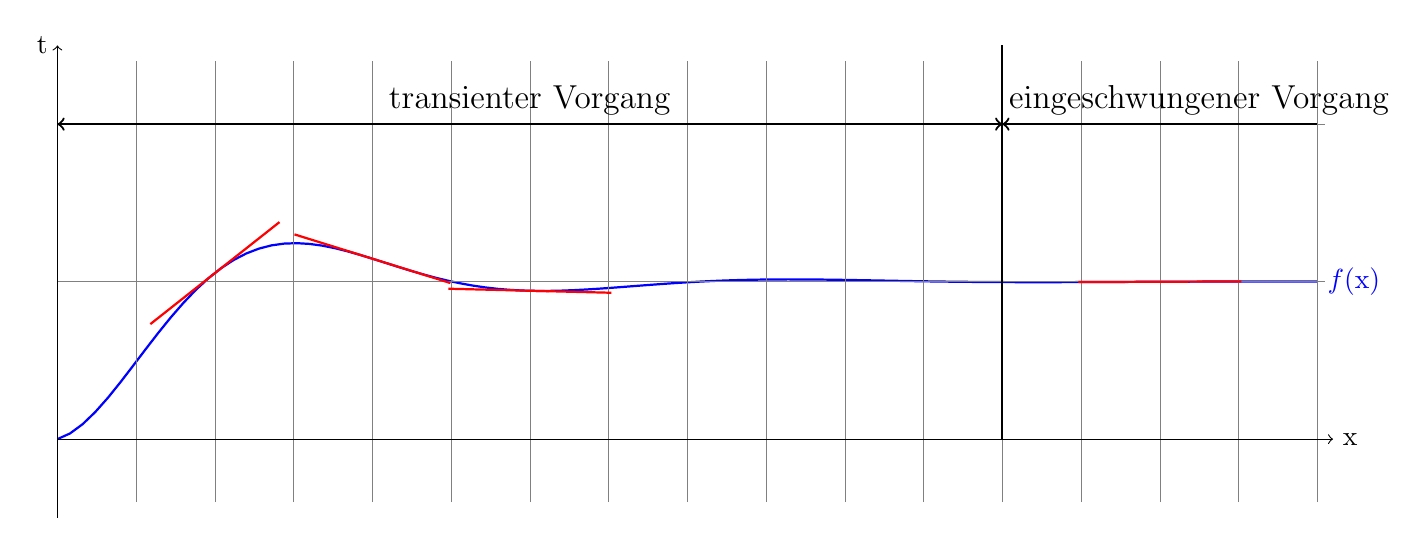
\begin{tikzpicture}[yscale=2,domain=0:16,samples=101,
pics/tangent at/.style={code={
    \path[name path=l] (#1*1cm-1pt,0|-current bounding box.south)
      -- (#1*1cm-1pt,0|-current bounding box.north);
    \path[name path=r] (#1*1cm+1pt,0|-current bounding box.south)
      -- (#1*1cm+1pt,0|-current bounding box.north);
    \draw[pic actions,
        name intersections={of=\pgfkeysvalueof{/tikz/tangent pic/graph name} and l,by=li},
        name intersections={of=\pgfkeysvalueof{/tikz/tangent pic/graph name} and r,by=ri}]
       (li) -- (ri);}},
tangent pic/.cd,graph name/.initial=graph]
      \draw[blue,thick,name path=graph] plot (\x,{1-exp(-0.45*\x)*(cos(deg(sqrt(1-0.0001)*\x))+0.3/(sqrt(1-0.2^2))*sin(deg(sqrt(1-0.1^2)*\x)))}) node[right] {$f(\mathrm{x})$};
      \draw[very thin,gray] (0,-0.4) grid (16.1,2.4);
      \draw[->] (0,0) -- (16.2,0) node[right] {$\mathrm{x}$};
      \draw[->] (0,-0.5) -- (0,2.5) node[left] {$\mathrm{t}$};
      \draw[black,<->,thick] (0,2) -- (12,2);
      \draw[black,thick] (6,2.15) node{{\large $\mathrm{transienter}\,\,\mathrm{Vorgang}$}};
      \draw[black,<-,thick] (12,2) -- (16,2);
      \draw[black,thick] (14.5,2.15) node{{\large $\mathrm{eingeschwungener}\,\,\mathrm{Vorgang}$}};
      \draw[black,-,thick] (12,2.5) -- (12,0); 
      \path foreach \X in {2,4,6,14}
      {pic[red,thick,shorten <=-1cm,shorten >=-1cm]{tangent at=\X}};
\end{tikzpicture}


%         \begin{tikzpicture}[domain=1.5:4.1,samples=101,
%         pics/tangent at/.style={code={
%                         \path[name path=l] (#1*1cm-1pt,0|-current bounding box.south)
%                         -- (#1*1cm-1pt,0|-current bounding box.north);
%                         \path[name path=r] (#1*1cm+1pt,0|-current bounding box.south)
%                         -- (#1*1cm+1pt,0|-current bounding box.north);
%                         \draw[pic actions,
%                         name intersections={of=\pgfkeysvalueof{/tikz/tangent pic/graph name} and l,by=li},
%                         name intersections={of=\pgfkeysvalueof{/tikz/tangent pic/graph name} and r,by=ri}]
%                         (li) -- (ri);}},
%         tangent pic/.cd,graph name/.initial=graph]
%         %\clip (-1,-3) rectangle ++ (10,10);
%         \draw[blue,thick,name path=graph] plot (\x,{\x^3-7.7*\x^2+19.2*\x-15.5}) node[right] {$f(\mathrm{x})$};
%         %\draw[very thin,gray] (-1,-3) grid (10,10);
%         \draw[->] (0,0) -- (5,0) node[right] {$\mathrm{x}$};
%         \draw[->] (0,-0.5) -- (0,3.5) node[left] {$\mathrm{y}$};        
%         \path pic[red,shorten <=-2cm,shorten >=-1cm]{tangent at=4};
% %       \path foreach \X in {4}
% %       {pic[red,thick,shorten <=-1cm,shorten >=-1cm,dashed]{tangent at=\X}};
%         \end{tikzpicture}
\end{document}
%%% Local Variables:
%%% mode: latex
%%% TeX-master: t
%%% End:
